\documentclass[svgnames,11pt]{beamer}
\input{/home/tof/Documents/Cozy/latex-include/preambule_commun.tex}
\input{/home/tof/Documents/Cozy/latex-include/preambule_beamer.tex}
%\usepackage{pgfpages} \setbeameroption{show notes on second screen=left}
\author[]{Christophe Viroulaud}
\title{Additionneur}
\date{\framebox{\textbf{Archi 06}}}
%\logo{}
\institute{Première - NSI}

\begin{document}
\begin{frame}
    \titlepage
\end{frame}
\begin{frame}
    \frametitle{}

    À partir des \emph{briques élémentaires} il est possible de construire des circuits plus complexes et ainsi permettre d'effectuer différentes opérations.

\end{frame}
\begin{frame}
    \frametitle{}

    \begin{center}
        \begin{framed}
            Comment construire un circuit permettant d'effectuer des additions?
        \end{framed}
    \end{center}

\end{frame}
\section{Notations booléennes}
\begin{frame}
    \frametitle{Notations booléennes}

    \begin{itemize}
        \item $\lnot$ pour NOT
        \item $\land$ pour AND
        \item $\lor$ pour OR
        \item $\oplus$ pour XOR
    \end{itemize}

\end{frame}
\begin{frame}
    \frametitle{}

    \begin{center}
        \begin{tabular}{|c|c|}
            \hline
            x & $\lnot x$ \\
            \hline
            1 & 0         \\
            \hline
            0 & 1         \\
            \hline
        \end{tabular}
        \captionof{table}{Table de vérité de $\lnot x$}
    \end{center}


\end{frame}
\begin{frame}
    \frametitle{}

    \begin{center}
        \begin{tabular}{|c|c|c|}
            \hline
            x & y & $x\lor y$ \\
            \hline
            0 & 0 & 0         \\
            \hline
            0 & 1 & 1         \\
            \hline
            1 & 0 & 1         \\
            \hline
            1 & 1 & 1         \\
            \hline
        \end{tabular}
        \captionof{table}{Table de vérité de $x\lor y$}
    \end{center}

\end{frame}
\begin{frame}
    \frametitle{}

    \begin{activite}
        Écrire les tables de vérités de $x\land y$ et $x\oplus y$.
    \end{activite}

\end{frame}
\begin{frame}
    \frametitle{}

    \begin{center}
        \begin{tabular}{|c|c|c|}
            \hline
            x & y & $x\land y$ \\
            \hline
            0 & 0 & 0          \\
            \hline
            0 & 1 & 0          \\
            \hline
            1 & 0 & 0          \\
            \hline
            1 & 1 & 1          \\
            \hline
        \end{tabular}
    \end{center}

\end{frame}
\begin{frame}
    \frametitle{}

    \begin{center}
        \begin{tabular}{|c|c|c|}
            \hline
            x & y & $x\oplus y$ \\
            \hline
            0 & 0 & 0           \\
            \hline
            0 & 1 & 1           \\
            \hline
            1 & 0 & 1           \\
            \hline
            1 & 1 & 0           \\
            \hline
        \end{tabular}
    \end{center}

\end{frame}

\begin{frame}
    \frametitle{}

    \begin{activite}
        \begin{enumerate}
            \item On définit 3 paramètres: $x,y,z$. Combien de combinaisons peut-on réaliser?
            \item Écrire la table de vérité de $x\land y \land z$.
        \end{enumerate}
    \end{activite}

\end{frame}
\begin{frame}
    \frametitle{}

    \begin{center}
        \begin{tabular}{|c|c|c|c|}
            \hline
            x & y & z & $x\land y \land z$ \\
            \hline
            0 & 0 & 0 & 0                  \\
            \hline
            0 & 0 & 1 & 0                  \\
            \hline
            0 & 1 & 0 & 0                  \\
            \hline
            0 & 1 & 1 & 0                  \\
            \hline
            1 & 0 & 0 & 0                  \\
            \hline
            1 & 0 & 1 & 0                  \\
            \hline
            1 & 1 & 0 & 0                  \\
            \hline
            1 & 1 & 1 & 1                  \\
            \hline
        \end{tabular}
    \end{center}


\end{frame}
\begin{frame}
    \frametitle{}

    \begin{activite}Écrire la table de vérité de $x\land (y \lor z)$.
    \end{activite}

\end{frame}
\begin{frame}
    \frametitle{}

    \begin{center}
        \begin{tabular}{|c|c|c|c|}
            \hline
            x & y & z & $y \lor z$ \\
            \hline
            0 & 0 & 0 & 0                  \\
            \hline
            0 & 0 & 1 & 1                 \\
            \hline
            0 & 1 & 0 & 1                  \\
            \hline
            0 & 1 & 1 & 1                 \\
            \hline
            1 & 0 & 0 & 0                  \\
            \hline
            1 & 0 & 1 & 1                 \\
            \hline
            1 & 1 & 0 & 1                 \\
            \hline
            1 & 1 & 1 & 1                  \\
            \hline
        \end{tabular}
    \end{center}


\end{frame}
\begin{frame}
    \frametitle{}

    \begin{center}
        \begin{tabular}{|c|c|c|c|c|}
            \hline
            x & y & z & $y \lor z$&$x \land (y \lor z)$ \\
            \hline
            0 & 0 & 0 & 0 &0                 \\
            \hline
            0 & 0 & 1 & 1     &0            \\
            \hline
            0 & 1 & 0 & 1   &0               \\
            \hline
            0 & 1 & 1 & 1  &0               \\
            \hline
            1 & 0 & 0 & 0   &0               \\
            \hline
            1 & 0 & 1 & 1  &1               \\
            \hline
            1 & 1 & 0 & 1   &1              \\
            \hline
            1 & 1 & 1 & 1  &1                \\
            \hline
        \end{tabular}
    \end{center}


\end{frame}
\begin{frame}
    \frametitle{}

    \begin{activite}
    Écrire la table de vérité de $(x\land y)\oplus (\lnot y \lor z)$
    \end{activite}

\end{frame}
\begin{frame}
    \frametitle{}

    \begin{center}
        \begin{tabular}{|*7{c|}}
        \hline 
        x & y & z & $(x\land y)$ & $\lnot y$ & $(\lnot y \lor z)$\\ 
        \hline 
0 & 0 & 0 &0&1&1\\
\hline 
0 & 0 & 1 &0&1&1\\
\hline 
0 & 1 & 0 &0&0&0\\
\hline 
0 & 1 & 1 &0&0&1\\
\hline 
1 & 0 & 0 &0&1&1\\
\hline 
1 & 0 & 1 &0&1&1\\
\hline 
1 & 1 & 0 &1&0&0\\
\hline 
1 & 1 & 1 &1&0&1\\
\hline
        \end{tabular}
        \end{center}

\end{frame}
\begin{frame}
    \frametitle{}

    \begin{center}
        \begin{tabular}{|*8{c|}}
        \hline 
        x & y & z & $(x\land y)$ & $\lnot y$ & $(\lnot y \lor z)$&$(x\land y)\oplus (\lnot y \lor z)$\\ 
        \hline 
0 & 0 & 0 &0&1&1&1\\
\hline 
0 & 0 & 1 &0&1&1&1\\
\hline 
0 & 1 & 0 &0&0&0&0\\
\hline 
0 & 1 & 1 &0&0&1&1\\
\hline 
1 & 0 & 0 &0&1&1&1\\
\hline 
1 & 0 & 1 &0&1&1&1\\
\hline 
1 & 1 & 0 &1&0&0&1\\
\hline 
1 & 1 & 1 &1&0&1&0\\
\hline
        \end{tabular}
        \end{center}

\end{frame}
\section{Demi-additionneur}
\begin{frame}
    \frametitle{Demi-additionneur}

    Un demi-additionneur prend deux bits en entrée $e_0$ et $e_1$ et renvoie la somme $e_0+e_1$ en sortie $s$. Il faut prendre en compte une éventuelle retenue $c$.

\end{frame}
\begin{frame}
    \frametitle{}

    \begin{center}
        \begin{tabular}{|cc||cc|}
        \hline 
        $e_0$ & $e_1$ & s & c \\ 
        \hline 
        0 & 0 & 0 & 0 \\ 
        \hline 
        0 & 1 & 1 & 0\\ 
        \hline 
        1 & 0 & 1 & 0\\
        \hline 
        1 & 1 & 0 & 1\\
        \hline 
        \end{tabular}
        \captionof{table}{Table de vérité du demi-additionneur}
        \end{center}

\end{frame}
\begin{frame}
    \frametitle{}
    \begin{center}
        \begin{tabular}{|cc||cc|}
            \hline 
            $e_0$ & $e_1$ & s & c \\ 
            \hline 
            0 & 0 & 0 & 0 \\ 
            \hline 
            0 & 1 & 1 & 0\\ 
            \hline 
            1 & 0 & 1 & 0\\
            \hline 
            1 & 1 & 0 & 1\\
            \hline 
            \end{tabular}
    \end{center}
    \begin{activite}
        \begin{enumerate}
        \item Quelles fonctions logiques reconnaît-on en \emph{s} et \emph{c}?
        \item En déduire le schéma du demi-additionneur.
        \end{enumerate}
        \end{activite}

\end{frame}
\begin{frame}
    \frametitle{}
    \begin{center}
        \begin{tabular}{|cc||cc|}
            \hline 
            $e_0$ & $e_1$ & s & c \\ 
            \hline 
            0 & 0 & 0 & 0 \\ 
            \hline 
            0 & 1 & 1 & 0\\ 
            \hline 
            1 & 0 & 1 & 0\\
            \hline 
            1 & 1 & 0 & 1\\
            \hline 
            \end{tabular}
    \end{center}
    {\Large $$s=e_0\oplus e_1$$
$$c=e_0\land e_1$$}

\end{frame}
\begin{frame}
    \frametitle{}

    \begin{center}
    \centering
    
\includegraphics[width=8cm]{ressources/demi-add.png}
    \captionof{figure}{Demi-additionneur}
    \label{IMG}
    \end{center}

\end{frame}
\section{Additionneur}
\begin{frame}
    \frametitle{Additionneur}

    Dans une addition bit à bit il faut prendre en compte l'éventuelle retenue de l'addition précédente. Ainsi un additionneur prend trois entrées $e_0$, $e_1$ et la retenue précédente $c_0$. Il renvoie une sortie $s=e_0+e_1+c_0$ et une retenue éventuelle $c$.

\end{frame}
\begin{frame}
    \frametitle{}

    \begin{activite}
    Compléter la table de vérité de l'additionneur.
    \begin{center}
        \begin{tabular}{|c|c|c||c|c|}
            \hline
            $e_0$ & $e_1$ & $c_0$ & s&c \\
            \hline
            0 & 0 & 0 &  &                 \\
            \hline
            0 & 0 & 1 &      &            \\
            \hline
            0 & 1 & 0 &    &               \\
            \hline
            0 & 1 & 1 &   &              \\
            \hline
            1 & 0 & 0 &    &              \\
            \hline
            1 & 0 & 1 &   &               \\
            \hline
            1 & 1 & 0 &   &             \\
            \hline
            1 & 1 & 1 &  &               \\
            \hline
        \end{tabular}
    \end{center}
    \end{activite}
\end{frame}
\begin{frame}
    \frametitle{}

    \begin{center}
        \begin{tabular}{|c|c|c||c|c|}
            \hline
            $e_0$ & $e_1$ & $c_0$ & s&c \\
            \hline
            0 & 0 & 0 & 0 &      0           \\
            \hline
            0 & 0 & 1 &  1    &   0         \\
            \hline
            0 & 1 & 0 &  1  &    0           \\
            \hline
            0 & 1 & 1 &  0 &     1         \\
            \hline
            1 & 0 & 0 &  1  &    0          \\
            \hline
            1 & 0 & 1 &  0 &     1          \\
            \hline
            1 & 1 & 0 &  0 &     1        \\
            \hline
            1 & 1 & 1 &  1&      1         \\
            \hline
        \end{tabular}
    \end{center}

\end{frame}
\begin{frame}
    \frametitle{}

    On peut remarquer:
    {\Large $$s=e_0\oplus e_1 \oplus c_0$$
    $$(e_0 \land e_1)\lor (e_0\land c_0)\lor (e_1\land c_0)$$}

\end{frame}
\begin{frame}
    \frametitle{}

    \begin{center}
    \centering
    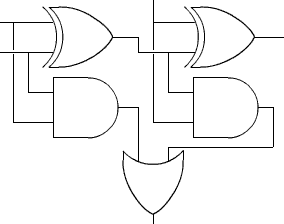
\includegraphics[width=7cm]{ressources/additionneur.png}
    \captionof{figure}{Additionneur}
    \label{IMG}
    \end{center}
\begin{activite}
Placer les entrées $e_0, e_1 c_0$ et les sorties $s,c$ sur le schéma.
\end{activite}
\end{frame}
\end{document}